\documentclass[11pt,titlepage]{article}
\usepackage[utf8]{inputenc}
\usepackage{fullpage}
\usepackage{enumerate}
\usepackage{graphicx}
\usepackage{apacite}
\usepackage{natbib}
\usepackage[]{algorithm2e}
\usepackage{array}

\usepackage{amssymb}
\usepackage{amsmath}

\usepackage{listings}
\usepackage{color}
\lstset{
basicstyle=\small\ttfamily,
columns=flexible,
breaklines=true
}

\lstdefinelanguage{diff}{
  morecomment=[f][\color{blue}]{@@},     % group identifier
  morecomment=[f][\color{red}]-,         % deleted lines 
  morecomment=[f][\color{green}]+,       % added lines
  morecomment=[f][\color{magenta}]{---}, % Diff header lines (must appear after +,-)
  morecomment=[f][\color{magenta}]{+++},
}

\title{Duplicate Aware Scheduling}
\author{Joshua Pfosi \& Nitesh Gupta}
\date{} 

\renewcommand*\contentsname{Table of Contents}

\usepackage{tocloft}
\renewcommand{\cftbeforesubsecskip}{10pt}

\begin{document}
\maketitle

\tableofcontents
\listoffigures
\listoftables

\pagebreak

\maketitle

\section{Introduction}

A common technique for application scalability at Internet-sized proportions is
distributed systems of computers which communicate over some network. By
leveraging the collective computing power of many machines, requests can be
served far faster than even the most powerful single cores. A classic example of
this paradigm is load balancing. Load balancing is an attempt to distribute
workloads across multiple resources to reduce latency and maximize throughput. A
load balancer is logically centralized entity which accepts incoming service
requests and maps them to a distributed network of servers in such a way as to
minimize average load on each server. There exist many load balancing algorithms
such as random, round robin, power of n choice etc. Each scheme excels under
different request patterns or workloads and is suboptimal or inadequate for
others. This manifests as a skewing of load (requests / sec) across servers.
Incoming requests to a heavily loaded server are, by definition, served less
quickly. This results in what are known as “stragglers”, or portions of a
distributed request which stall the entire request as they were erroneously
directed to a heavily loaded server. While load balancers attempt to reduce the
likelihood of stragglers, this work attempts to minimize the effects of them.

The concept is to reduce the effects of poorly routed primary requests by
sending multiple instances, or duplicates, of that request to different servers.
If done carefully, the set of requests (the primary and the duplicates) will not
all be directed to loaded servers. Therefore, at least one will be served in the
expected amount of time, and a straggler will not hold up an entire request.
Clearly, by doubling or tripling network traffic naively, this technique would
increase server load significantly and be counterproductive. To meet this
challenge, we propose duplicate aware scheduling. That is, proper
instrumentation of specific load-sensitive applications to understand and
prioritize primary and duplicate requests differently so that stragglers are
minimized but duplicate requests are not served before primaries. We hypothesize
that by reducing the effects of stragglers on extremely loaded servers, an
increase in throughput and a decrease in average latency will be observed.

\section{Experimental Setup}

To verify the hypothesis, we required a method to create large and diverse
workloads as well as a typical application to instrument. Fortunately, Yahoo!
Cloud Serving Benchmark (YCSB) provided a workload generator for database stores
which was sufficiently robust from which we could work. We chose Memcached as
the application to instrument. Memcached is a distributed memory object caching
system implemented as a in-memory key-value store~\citep{memcached}. We selected
it for its relatively simple high level design and lack of replication strategy.
Memcached is also built upon an event notification library, libevent, which
implements a priority API which met our desired priority semantics.

\subsection{Top Level Diagram}\label{top_level_diagram}

Fig.~\ref{tld}, below, presents the high level design for our experiments. YCSB
behaves logically as one client but may be distributed among multiple physical
computers to achieve desired server loads. Memcached is run independently on
four different servers without a backend database layer. Each server is
responsible for a fourth of the primary key space, and a fourth of the duplicate
key space. With carefully chosen hash functions, the mass majority of duplicate
and primary mappings should be distinct for a given key.

\begin{figure}[h!]
  \centering
  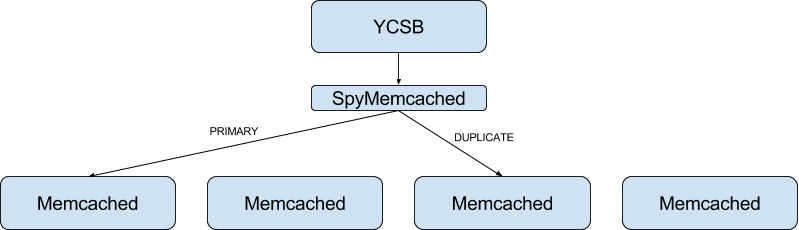
\includegraphics[width=\textwidth]{tld.png}
  \caption[Top level diagram]{Top level diagram of overall modules}
  \label{tld}
\end{figure}

YCSB generates a workload, then a Java Memcached client, Spymemcached,
implements the requests to Memcached servers. A requested key is hashed to
choose a memcached instance to fulfill that request. Without modification,
Spymemcached accepts a list of Memcached hosts and creates TCP connections to
those hosts. Requests are hashed consistently via a selected hash function and
the response is returned synchronously to YCSB which benchmarks the transaction.
Throughput and latency statistics are aggregated and output by YCSB.

\subsection{Duplicate Awareness}

This work modifies both Spymemcached and Memcached to be \textit{duplicate
aware}. This implies instrumenting the former to hash and send duplicate
requests distinctly from primary requests, and the latter to recognize and
prioritize a request as \textsc{primary} or \textsc{duplicate}. For every
\texttt{insert} operation a YCSB workload generates, the YCSB client
asynchronously makes two \texttt{set} requests to Spymemcached, one primary and
one duplicate. For every \texttt{read} operation, YCSB asynchronously makes two
\texttt{get} requests to Spymemcached, one primary and one duplicate. Once the
\texttt{get} or \textsc{set} resolve, YCSB cancels the remaining request and
returns. Therefore, if the \textsc{primary} request is lagging, the
\textsc{duplicate} request can reduce latency by resolving first.

\subsubsection{Yahoo! Cloud Serving Benchmark}

We use YCSB to create workloads to stress the duplcate aware memcached
instances. The critical use case in which duplicate aware scheduling shines is
in the presence of skewed workloads. That is, when one or more servers are
significantly more loaded than others. This allows duplicate requests, sent to
underutilized resources, to fulfill the otherwise blocked request. To verify we
have loaded the servers properly, we can leverage Memcached's \texttt{stats} API to
query for \texttt{get} and \texttt{set} operation totals for a given workload.
Comparing such plots with and without duplicate requests provides confidence
that the hashing algorithms are distributing requests appropriately. A latent
requirement for the utility of these graphs is a deterministic key sequence. By
inspecting YCSB source code, however, it appears an additively increasing
sequence starting at 0 is used by default. Therefore, the plots of requests per
server per workload are valid.

\subsubsection{Spymemcached}

Spymemcached uses \texttt{getNodeForKey} to hash a key and return a
\texttt{MemcachedNode}. Overwriting this method to hash \textsc{duplicate} keys
(i.e. \texttt{dupKey = ``dup\_\_'' + key}) differently is sufficient to
distribute the duplicate load differently.  The code changes to implement this
change are small and can be found in Appendix~\ref{app:spymemcached}.

\subsubsection{Memcached}

Memcached, on the other hand, was slightly more complex.  Memcached listens for
incoming connections in a master thread and dispatches new connections in a
round robin fashion to a fixed number (typically 4) of worker threads. Each
worker, in turn, listens for traffic on each of its open connections and
transitions through a state machine based on incoming requests.  The
``listening'' construct is implemented via Libevent which supports an event
callback for configurable triggers on file descriptors. Memcached uses this to
poll for actionable events on the TCP sockets of each worker thread.  This way
each worker thread sees a synchronized, serialized queue of requests to which it
responds. Without modification, Memcached treats all incoming requests
equivalently. To make it duplicate aware, however, requires a priority queue
where \textsc{primary} requests are served before \textsc{duplicate}s. Libevent
allows a client to prioritize specific events over others. Events can be
distinguished only by the file descriptor to which they are associated or the
event flags for which they activate~\citep{libevent_priority}. As we are strictly
using \textsc{ev\_read}, we must use separate file descriptors and therefore
distinct TCP connections for \textsc{primary} versus \textsc{duplicate}
requests. A simple way to accomplish this is to leverage Memcached existing
dispatching algorithm, round robin, and hardcode that the events on the first
connection given to any worker thread are high priority, and every subsequent
connection's events are low priority. The code changes to implement this change
are small and can be found in Appendix~\ref{app:memcached}.

\subsection{Emulab}

For consistency, all experiments were conducted on a networked testbed called
Emulab, on Ubuntu 14.04 LTS (64-bit), over a 10Gb LAN (as in
Fig.~\ref{topology}). The experiment was entitled \texttt{dup} on the
\texttt{comp150} project. See Appendix~\ref{app:tcl} for the NS script which
constructed the desired topology.

\begin{figure}[h!]
  \centering
  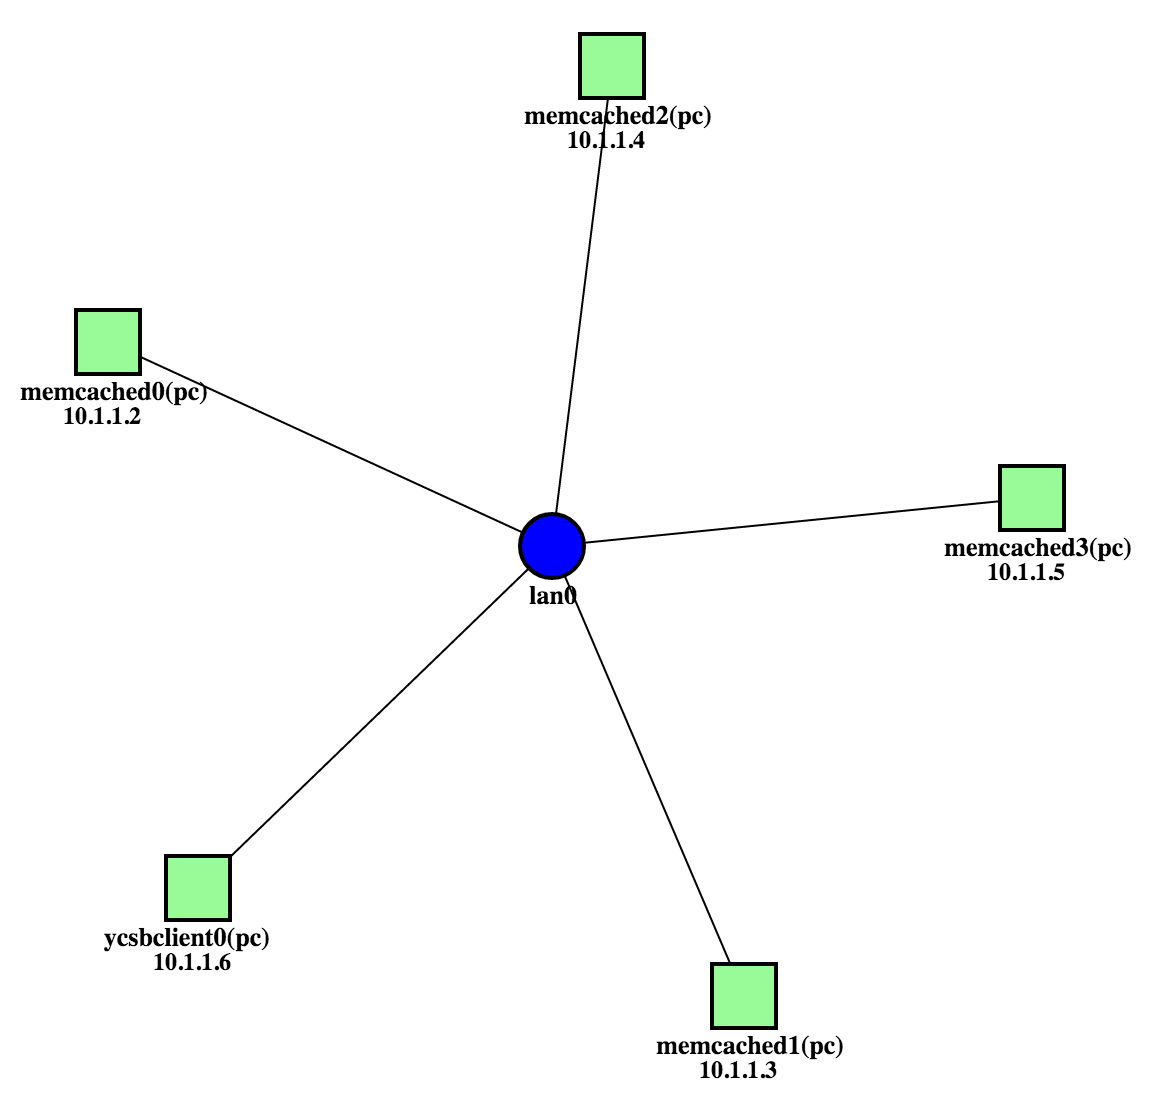
\includegraphics[width=0.3\textwidth]{topology.png}
  \caption[Emulab topology]{Emulab topology}
  \label{topology}
\end{figure}
 
\section{Experimental Execution}

The execution of experiments is entirely scripted. YCSB is prebuilt with each
duplicate scheme in directories \texttt{YCSB\_unaware} and \texttt{YCSB\_aware}
for control and scheduled duplicates, respectively. Running \texttt{sh
run-experiments.sh} executes a number of trials of each of these test cases on
all workloads under the YCSB workload directory for multiple request sizes.
Specifically, 1000 records were loaded, and 10000 operations were executed.
Record sizes were 1 kB and 5 kB. These values were selected to allow the
experiments to run in a reasonable amount of time, and should be tweaked by
future researchers.

\subsection{Utilities}

In addition, there are many provided utilities, summarized in
Table~\ref{utilities}.

\begin{table}[h!]
  \resizebox{\linewidth}{!}{
    \begin{tabular} {|l||p{8cm}|}
      \hline
      Usage & Description\\\hline
      \texttt{sh kill-experiment.sh <NUM\_CLIENTS> <NUM\_SERVERS>} & Kills all
      running \texttt{memcached} and \texttt{ycsb} instances on all Emulab
      machines.\\\hline
      \texttt{sh build-\{memcached,ycsb,libevent\}.sh} & Compresses, copies,
      decompresses and builds the desired software on the appropriate Emulab
      machines.\\\hline
      \texttt{sh build-emulab.sh <NUM\_CLIENTS> <NUM\_SERVERS>} & After swap in,
      this command will install and build all dependencies and software to run
      experiments.\\\hline
      \texttt{sh run-experiments.sh} & Runs all types of experiments through a
      variety of parameters and outputs data to subdirectories for
      analysis.\\\hline
      \texttt{sh make-dup-aware.sh} & Compiles \texttt{memcached} to be duplicate
      aware on the appropriate Emulab machines.\\\hline
      \texttt{sh run-experiments.sh} & Runs all experiments for a variety of
      parameters.\\\hline
      \texttt{sh plot-\{load,throughput\}.sh <XLABEL> <YLABEL> <TITLE> <DATA> <OUTPUT>} &
      Generates basic scatter plots.\\\hline
    \end{tabular}
  }
  \caption{Summarizes utilities provided as scripts}
  \label{utilities}
\end{table}

\section{Results}

Using the setup from Fig.~\ref{topology}, a single YCSB client made requests to
four Memcached instances and recorded throughput. To test the efficacy
of duplicate aware scheduling, we developed a set of workloads and measured the
throughput and latency with and without duplicate aware scheduling as a
function of load (i.e. YCSB \texttt{fieldlength}). Fig.~\ref{load}
illustrate the load on each server for the control (black points) as well as
with \textsc{duplicate} requests (yellow points).


Fig.~\ref{throughput} depicts the variance in throughput seen under duplicate
aware scheduling. We expected duplicate requests to reduce the effects of
stragglers and therefore increase throughput. In some instances, this is
observed, however, this is likely due to sampling error. With such low
throughput numbers (typical Memcached systems see on the order of tens or
hundreds of thousands), statistical variance in throughput obscures our results
significantly.

\section{Future Work}

This work laid the ground work for future experimentation with Memcached and
duplicate aware scheduling. We used a straightforward and naive duplicate
scheduling technique. Future work could benefit from using other techniques such
as dynamically sending \textsc{duplicate} packets based on measured load of a
given server.

Additionally, this work was majorly compromised by inexplicably low throughput on
the Memcached servers. This reduces the resolution of our results and the
feasibility of testing. Switching to another load generator or testbed to
improve throughput and reduce latency may demonstrate the true efficacy of
duplicate aware scheduling.

Finally, for simplicity we only used four Memcached servers and a single client.
While sufficient, spreading load over multiple servers would exaggerate the
skewing effect of the \texttt{latest} request distribution of YCSB and therefore
illustrate the benefits of duplicate aware scheduling more clearly.

\section{Conclusion}

In conclusion, this paper contributes a robust, automated environment that,
combined with a remote testbed such as Emulab, can be used to experiment with
and verify predictions associated with duplicate aware scheduling.
Unfortunately, due to technical and logistical limitations, the original
hypothesis could neither be accepted nor refuted, but by leveraging the scripts
documented here, future work is better poised to do so.

\begin{figure}[h!]
  \centering
  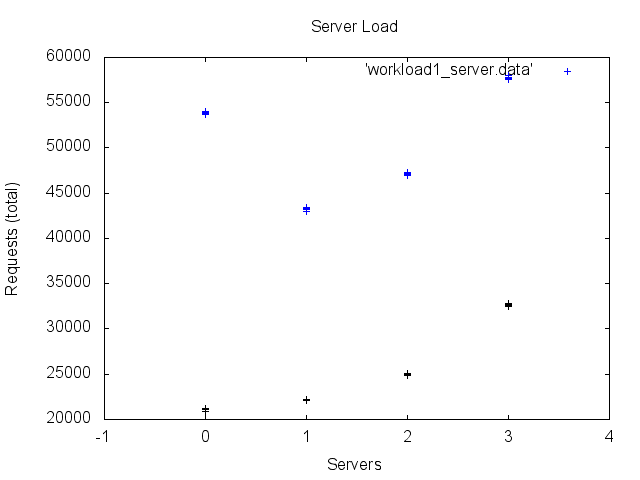
\includegraphics[width=0.35\textwidth]{workload1_load.png}
  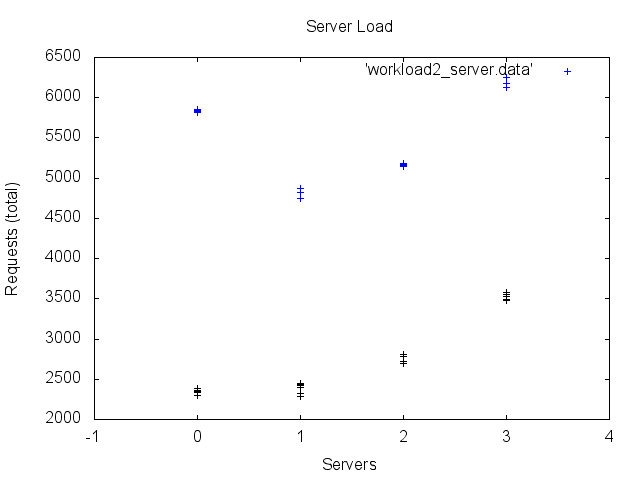
\includegraphics[width=0.35\textwidth]{workload2_load.png}
  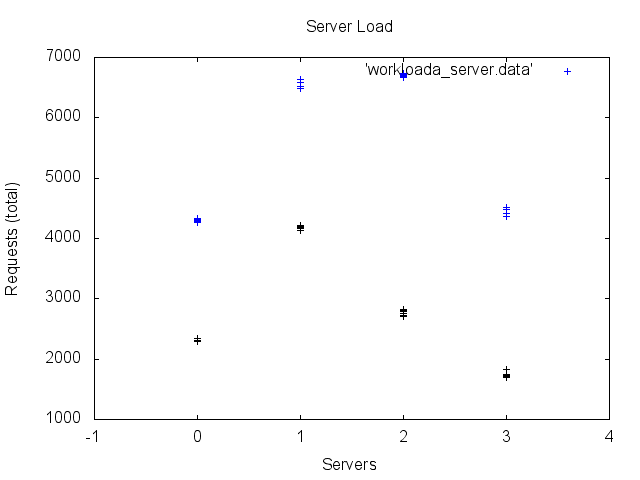
\includegraphics[width=0.35\textwidth]{workloada_load.png}
  \caption[Server load]{The servers' load for \textsc{primary}-only and
  \textsc{duplicate} requests. Load under, from right to left, workload 1, 2,
  and a. }
  \label{load}
\end{figure}
\begin{figure}[h!]
  \centering
  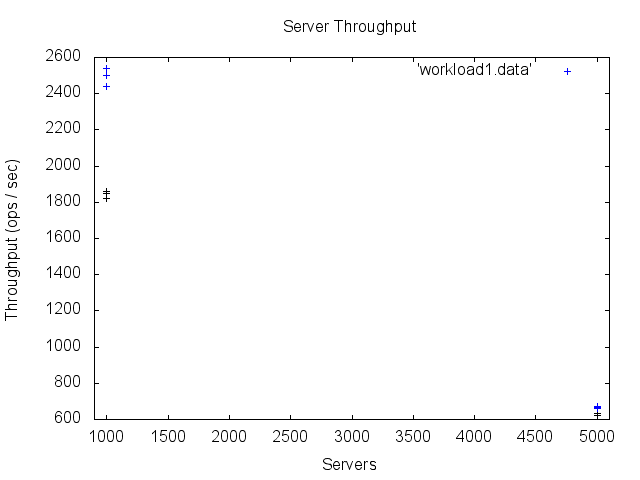
\includegraphics[width=0.35\textwidth]{workload1_throughput.png}
  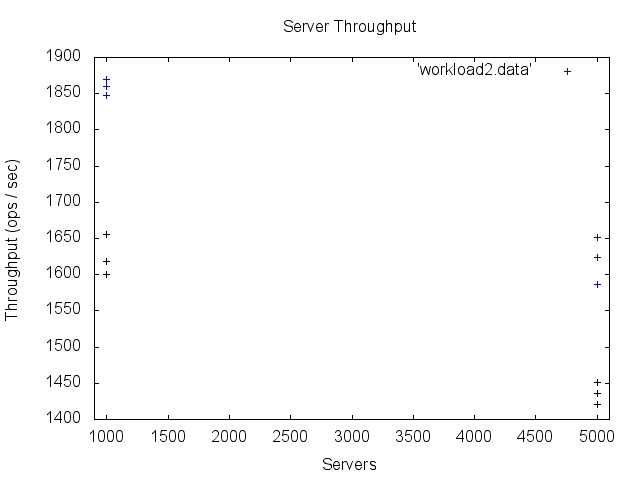
\includegraphics[width=0.35\textwidth]{workload2_throughput.png}
  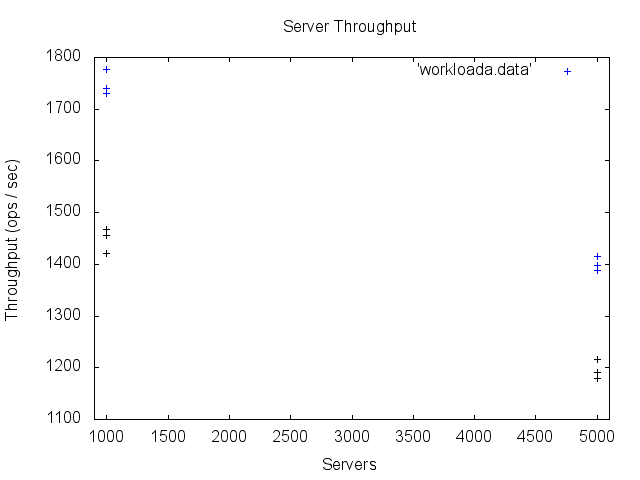
\includegraphics[width=0.35\textwidth]{workloada_throughput.png}
  \caption[Throughput]{The client's throughput as a function of record size for
  control and duplicate-aware (black and yellow, respectively).}
  \label{throughput}
\end{figure}

\pagebreak

\appendix
\section{\texttt{emulab.tcl}} \label{app:tcl}

\lstinputlisting[language=tcl]{emulab.tcl}

\section{Memcached Modifications} \label{app:memcached}

\lstinputlisting[language=diff]{memcached.diff}

\section{Spymemcached Modifications} \label{app:spymemcached}

\lstinputlisting[language=diff]{spymemcached.diff}

\pagebreak

\nocite{*}
\bibliographystyle{apacann}
\bibliography{final_report}

\end{document}
